\documentclass[sigconf]{acmart}
\usepackage[utf8]{inputenc}

\settopmatter{printacmref=false}
\renewcommand\footnotetextcopyrightpermission[1]{} % removes footnote with conference information in first column
\pagestyle{plain}

\usepackage{url}
\usepackage{hyperref}
\hypersetup{
    colorlinks=true,
    linkcolor=blue,
    filecolor=magenta,      
    urlcolor=cyan,
}
\urlstyle{same}


\usepackage{listings}
\usepackage{lipsum}

% Enabling Javascript syntax highlight in code snippet - BEGIN 
% https://tex.stackexchange.com/questions/89574/language-option-supported-in-listings
\usepackage{color}
\definecolor{lightgray}{rgb}{.9,.9,.9}
\definecolor{darkgray}{rgb}{.4,.4,.4}
\definecolor{purple}{rgb}{0.65, 0.12, 0.82}
\definecolor{darkgreen}{rgb}{0, .64, 0}

\lstdefinelanguage{JavaScript}{
  keywords={typeof, new, true, false, catch, function, return, null, catch, switch, var, if, in, while, do, else, case, break},
  keywordstyle=\color{blue}\bfseries,
  ndkeywords={class, export, boolean, throw, implements, import, this},
  ndkeywordstyle=\color{darkgray}\bfseries,
  identifierstyle=\color{black},
  sensitive=false,
  comment=[l]{//},
  morecomment=[s]{/*}{*/},
  commentstyle=\color{purple}\^amily,
  stringstyle=\color{darkgreen}\ttfamily,
  morestring=[b]',
  morestring=[b]"
}

\lstset{
   extendedchars=true,
   basicstyle=\footnotesize\ttfamily,
   showstringspaces=false,
   showspaces=false,
   tabsize=2,
   breaklines=true,
   showtabs=false,
   captionpos=b,
   frame=single,
   xleftmargin=0.5em,
   belowcaptionskip=0em
}

\setlength{\belowcaptionskip}{-1em}
% Enabling Javascript syntax highlight in code snippet - END

\newcommand{\APIName}{Successorships }
\newcommand{\APINameNoSpace}{Successorships}

\newcommand{\APIshort}{Shippy }
\newcommand{\rpm}{\raisebox{.2ex}{$\scriptstyle\pm$}}

\newcommand{\accessed}{accessed 2017-12-11}

\usepackage{array}
\newcolumntype{L}[1]{>{\raggedright\let\newline\\\arraybackslash\hspace{0pt}}m{#1}}
\newcolumntype{C}[1]{>{\centering\let\newline\\\arraybackslash\hspace{0pt}}m{#1}}
\newcolumntype{R}[1]{>{\raggedleft\let\newline\\\arraybackslash\hspace{0pt}}m{#1}}


\graphicspath{{figures/}{pictures/}{images/}{./}}

%opening
\title{Successorships - Fault-Tolerant Local WebApps}

\author{Arthur Marques \qquad Felix Grund \qquad Paul Cernek}
\affiliation{
    \institution{University of British Columbia}
    \city{Vancouver} 
    \state{BC} 
  }

\begin{document}

\begin{abstract}
As networking capabilities become more ubiquitous across different types of devices, applications that communicate over local area networks are becoming increasingly common.
This trend has been accelerated by the adoption of zero-configuration (zeroconf) networking standards that eliminate the burden of setup procedures.
Applications operating in zeroconf settings often face the challenge of maintaining reliability and consistency in the face of wireless links and mobile devices, resulting in potentially intermittent connectivity between hosts.
Fault-tolerance is thus a desirable property for such applications, but it can be difficult to achieve in practice.
To this end, we introduce Successorships, a JavaScript library that provides the appealing qualities of zeroconf enriched with fault-tolerance, to applications running in the browser.
Our library enables graceful recovery after server failure by handing over the server role to one of the clients currently in the network.
We evaluate our approach with a sample application, focusing on usage scenarios that involve interactions between users in a small mobile network. 
We find that our library recovers from failures gracefully with an average of 15 seconds and that application state is maintained with eventual consistency.
\end{abstract}

\maketitle

\section{Introduction}
\label{sec:introduction}

Throughout the last decade we have seen the Internet become the most commonly used infrastructure for communication. Regardless of physical location, people and their devices communicate via messengers and VoIP, and collaborate via live editing tools such as Google Docs, Sheets, and, Slides. 
At the same time, we have seen the paradigm of applications communicating over local area networks become increasingly common for certain scenarios like home entertainment (e.g. Google Chromecast, Apple Bonjour, Spotify Connect) or Wi-Fi printers. 
With the advancements of ``smart'' devices and the ``Internet of Things'' (IoT) it is likely that this trend will grow beyond these currently still narrowly scoped application domains.

The adoption of standards that eliminate the burden of manual configuration of network devices further contributes to this movement. One such standard that has received widespread usage is Zero-configuration networking~\cite{guttman_2001} and its protocols mDNS~\cite{cheshire_2013_mdns} for service advertisement and DNS-SD for service discovery~\cite{cheshire_2013_dnssd}.
Using the \textit{Zeroconf} protocols, devices can publish named services in the local network and discover such services automatically in an ad-hoc fashion.
While most applications for Zeroconf networks are shipped with specific hardware (e.g. Google Chromecast dongle) there have recently been attempts to provide software environments for developers to enable them write their own applications on already existing hardware infrastructure.
One such application was Mozilla FlyWeb\footnote{https://wiki.mozilla.org/FlyWeb}, an addon for the Firefox browser that made it possible to advertise and discover services from within Web applications through a JavaScript API.
In a previous project, we created \textit{Successorships}~\footnote{https://github.com/ataraxie/successorships}, a JavaScript library exposing an easy-to-use API to build fault-tolerant Zeroconf web applications.
Successorships was built on top of Mozilla Flyweb as one main part of its architecture.
This decision confronted us with significant problems:
\begin{itemize}
    \item FlyWeb had been declared abandoned by Mozilla even before we finished our work on our library.
    \item The implementation of the Zeroconf protocols in FlyWeb was slow to a degree that made our library fairly unusable in practice.
    \item FlyWeb contained a bug that made our library usable on MacOS only.
\end{itemize}

To overcome our troubles in Successorships, we introduce Zeroties (zero ties), a platform-independent asynchronous publish/subscribe service for Zeroconf advertisement and discovery.
We carefully reviewed different publish/subscribe designs~\cite{eugster_2003} and implemented a communication scheme based on \textit{asynchronous notifications}.
The operations exposed by Zeroties are as follows:
\begin{itemize}
    \item \textbf{Publish}: publish a Zeroties service and advertise it in the local network
    \item \textbf{Subscribe}: listen for updates on the list of available Zeroties services
\end{itemize}

Zeroties ships with two components: (1) a standalone OS-level daemon, and (2) addons for Chrome and Firefox that connect to this daemon.
With our addon implementations for Chrome and Firefox we aim to show that our approach translates well between different browsers and does not share the restrictions of FlyWeb.
Our browser addons expose an API to web applications that comprises the full service/discovery functionality of Zeroconf.
As a result, we have successfully eliminated the ties that prevented Successorships from usage in practice.

To evaluate Zeroties, we first created the webapp-based presentation for this project using Successorships in combination with the Zeroties daemon and the addon for Google Chrome.
Running the presentation on Chrome proved that we successfully broke ties with FlyWeb and Mozilla Firefox.
Furthermore, we could get a first sense in this example application that recovery from failures was significantly faster than with the previous version based on FlyWeb.
To evaluate these findings empirically, we analyzed the changes in performance with a test scenario based on the evaluation framework from Successorships.
We simulated nine failures on a small network of 6 nodes, first with the old FlyWeb-based implementation and then with the new version based on Zeroties.
While recovery took on average 12.93 seconds with FlyWeb, it took only 1.55 seconds using Zeroties, indicating a speedup of nearly a factor of 10.

In summary, we make the following contributions:
\begin{itemize}
    \item Zeroties, a asynchronous standalone publish/subscribe service for Zeroconf applications.
    \item Addons for Chrome and Firefox that make this service available to web applications.
    \item An empirical evaluation based on a Zeroties sample application indicating significant performance improvements.
\end{itemize}

The remainder of this paper is organized as follows: Section~\ref{sec:background_and_motivation} provides some background and motivation on why the idea for Zeroties came to be. Section~\ref{sec:approach} presents the system model and design goals of Zeroties, before Section~\ref{sec:implementation} describes its implementation. We evaluate Zeroties in Section~\ref{sec:evaluation} and suggest limitations and future work in Section~\ref{sec:limitations_and_future_work}. Section~\ref{sec:related_work} situates our work in the context of related research and Section~\ref{sec:conclusion} concludes the paper.




\section{Background \& Motivation}
\label{sec:background}

Our work lies at the confluence of three distinct areas of networking and distributed systems: Zero-Configuration Networks (Zeroconf), in-browser Web servers, and fault tolerance.
Here we provide an overview of these topics.

\begin{figure}[h]
      \centering
      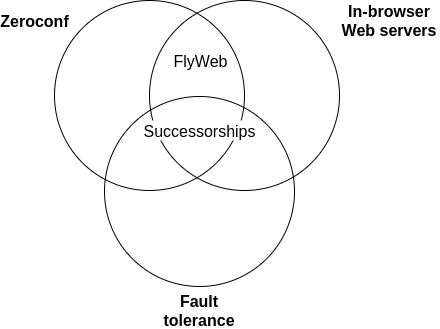
\includegraphics[keepaspectratio,width=6cm]{shippy-intersections}
      \label{fig:stack}
\end{figure}

\subsection{Zeroconf}
\label{sub:background_zeroconf}

Hosts connected to a network rely on maintaining a common consensus on such basic matters as addressing and name resolution, if they are to have any hope of communicating over that network.
This need is often fulfilled by specially-designated configuration servers, such as DHCP or DNS servers.
However, such servers can be absent in common networking situations, such as \textit{ad hoc} networks.
In such cases, it remains desirable for hosts to handle these matters in a seamless and cross-platform fashion, without the need for manual configuration.
This is the problem addressed by the group of protocols referred to as Zeroconf, short for ``Zero Configuration Networking''.\footnote{Although the term is sometimes used more broadly to designate any suite of technologies that seeks to address this problem, we observe the more specific meaning established by the former IETF Working Group by the same name.
See e.g. \url{http://www.zeroconf.org/}.}
Zeroconf protocols solve the problems of address allocation, address queries (mDNS), and network service discovery (DNS-SD), specifically when hosts share a direct link (be it logical or physical).
Since the first of these (address allocation) is a \textit{de facto} standard, as it has been integrated into consumer operating systems and printers since the early 2000s, we focus on the latter of these two here.

\textbf{Address queries.}
A name server can be used on a local network to maintain a mapping of logical names to IP addresses.
In the absence of such a server, a Zeroconf protocol called mDNS (short for ``multicast DNS'') can be used to formulate address queries on the local network.
As per its name, mDNS broadcasts these queries onto the local network rather than directing them to a single server; it also includes a mechanism to resolve naming conflicts~\cite{rfc6762}.
mDNS aims to handle any type of record lookup that could be handled by a DNS server, not just name-to-address lookups.
mDNS has grown steadily in popularity amongst networked devices; implementations of mDNS include Apple Bonjour, Spotify Connect, Philips Hue, Google Chromecast, and Avahi (an open-source implementation for Linux).

\textbf{Service discovery.}
Once connected to a network, a host may wish to learn about the services offered by the other devices connected to the network, such as printing or media streaming.
In a centrally-administered network, this may be accomplished by a directory server, such as a DNS server.
However, when such a server is lacking, the Zeroconf protocol called DNS-SD (``DNS service discovery'') leverages the ability to make distributed DNS queries provided by mDNS, to register, enumerate, and resolve local network services~\cite{rfc6763}.


\subsection{In-Browser Web Servers}
\label{sub:background_in_browser_web_servers}

More recently, a number of technologies have emerged to enable Web servers to be deployed entirely from within Web browsers.
Such technologies have the appeal that they simplify the process of serving Web content, thus potentially expanding the breadth of users capable of doing so.
For example, Opera Unite\footnote{\url{http://help.opera.com/Windows/12.10/en/unite.html}}, Web Server Chrome\footnote{\url{https://github.com/kzahel/web-server-chrome}}, PeerServer\footnote{\url{http://www.peer-server.com/}}, and FlyWeb\footnote{\url{http://flyweb.github.io/}} all enable browser applications to publish fully functioning Web servers.
We discuss FlyWeb below, and defer details on a few other approaches to Section \ref{sec:related_work}.

\subsection{The power of Zeroconf in the browser}
\label{sec:background_flyweb}

HTTP servers running on hosts that usually access the Web as clients face a few challenges not normally encountered by those running on dedicated server machines.
For example, they must be properly configured to circumvent firewalls, and they must ensure that other clients have a way of finding out their IP address.

The FlyWeb project, developed by the Mozilla Firefox community, addresses the problem of advertising and discovering in-browser Web services in the particular environment of local networks, by leveraging Zeroconf service advertisement and discovery.
To this end, FlyWeb provides two key pieces of functionality: 
\textit{(i)} an implementation of mDNS, allowing those services to advertise their name and address to peers on the local network, and 
\textit{(ii)} a FlyWeb service discovery menu, which uses a built-in implementation of DNS-SD to enumerate locally-discovered services.
The goal is for devices on a local network to be able to stream applications and content to one another using widely available Web technology.\footnote{\url{https://hacks.mozilla.org/2016/09/flyweb-pure-web-cross-device-interaction/}}
%FlyWeb was released in mid-2016, but is no longer actively maintained as of August 2017.

An important part of the appeal of this approach is its sheer versatility: it empowers any Web application with the ability to connect heterogeneous devices over an \textit{ad hoc} network, without each user needing to download a native app for their particular platform.
Examples of successful demonstrations of this idea include a collaborative photo sharing app, a printer interface, a temperature monitoring interface, and even a quadcopter controller.\footnote{\url{https://github.com/flyweb/examples}}


\subsection{The need for availability}
\label{sec:background_motivation}

A different challenge facing in-browser Web servers is that their availability is limited by that of the host machine.
Dedicated server machines usually have static network addresses and are often streamlined for serving Web content; however, the class of devices that can run a Web browser is much wider, including mobile devices, hence posing a novel challenge to service availability.
To the best of our knowledge, at the time of writing, none of the currently-existing technologies address the issue of recovering from disruptions of server availability for in-browser Web services.

We argue that application availability in the face of server failure is a requirement for many common use cases of client-server Web applications running on local networks.
This is especially true when one considers the current prevlance of networked mobile devices, where the server node might leave the local network, or fail due to other reasons such as low battery.

To motivate this concretely, consider a simple queuing Web application called \texttt{QueueApp}, which might be useful in the following scenario: a TA\footnote{Teaching Assistant} holds office hours in a small classroom, and students arrive at random intervals seeking individual assistance.
Students may arrive at a rate that exceeds that at which the TA is able to address their concerns, and so the TA wishes to keep track of the order in which they arrive.
The TA takes out her smartphone and loads \texttt{QueueApp}, which immediately starts a Web server on her phone.
As students arrive, she directs them to the URL of the local \texttt{QueueApp} service; when they connect, they are faced with an interface that enables them to either join the queue if they are not already in it, or to leave it if they are.
Now, say the TA needs to temporarily leave the room, for example to take an important phone call.
Unless special functionality is implemented by the application, the clients (students) will get disconnected from the server (TA), and the application state will need to be reset.

We argue that in such a case, it would be of great practical value for \texttt{QueueApp} to continue functioning seamlessly, even in the absence of the initial server.
What if 5 students enter the room while the TA is out?
In this paper, we make the case that those students should be able to enqueue despite the absence of the TA.

In the following section, we explain how we achieve this in the \APIName library.


\section{Approach}
\label{sec:approach}

\subsection{Environment and System Architecture}
\label{sub:architecture}

Figure~\ref{fig:architecture} illustrates the environment, placement of Zeroties, and the communication between components.
We describe the parts in the Figure by refering to the numbers in the ellipsis.

\begin{figure}[h]
    \centering
    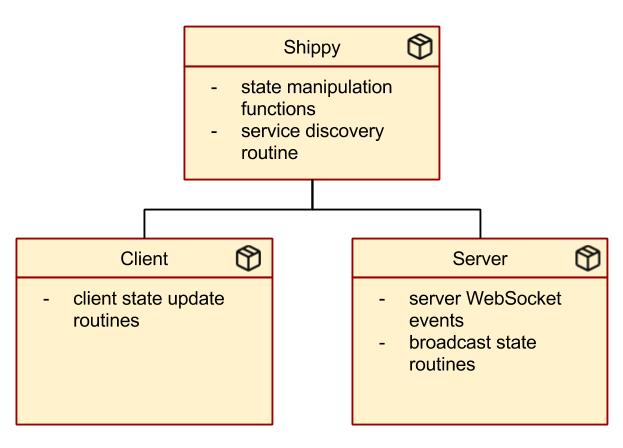
\includegraphics[keepaspectratio,width=6cm]{architecture}
    \caption{System architecture and environment in Zeroties.}
    \label{fig:architecture}
\end{figure}

\begin{enumerate}
\item \textbf{Router}~\footnote{Note that we use the term router somewhat casually in this context. Our notion of router is basically any part in the local network that serves the list of available Zeroconf services, as it can be obtained with DNS-SD. This may involve DHCP, IPv6 Router Advertisement Options or other mechanisms as specified on page 27f of~\cite{cheshire_2013_dnssd}. In other words, we simply call the component that stores the service list obtained from a DNS-SD-capable router.}: we use the protocols provided by Zeroconf (\cite{cheshire_2013_dnssd, cheshire_2013_mdns}) for Zeroties. 
In essence, this means that an authoritative list of currently available Zeroties services (as a subset of all Zeroconf services) can be obtained from the router at any given time.

\item \textbf{Hosts}: there can be an arbitrary number of hosts in our local network. A host can be any device in the network with an instance of Zeroties running (i.e. any device with an OS capable of Zeroconf/DNS-SD protocols).

\item \textbf{Zeroties Daemon}: the instance of Zeroties running on this device. 
This is an OS-level background application maintaining a list of services.
This list is a mirror of the service list obtained from the router by means of the Zeroconf protocols. 
The list of services constitutes the state of the distributed system\footnote{Note that there is a clear line between Successorships and Zeroties: Zeroties does not know about the arbitrarily complex state of Successorships or any other app that builds on Zeroties.}.
We originally intended to integrate this application into browser addons, but were restricted by browser policies.
In particular, there is no possibility to start a web server or publish a Zeroconf service from within a browser addon.
Hence our alternative solution of an OS-level app that communicates with our browser addons through stable bi-directional message channels.

\item \textbf{Browser Addons}: we require browser addons that mediate between web applications and the Zeroties daemon. These addons expose a JavaScript API to apps built on top of Zeroties.
We have implemented addons for Google Chrome and Mozilla Firefox that constitute such a mediator and we have run Successorships apps with these addons (see Section~\ref{sec:evaluation}).
These addons use Zeroties as a publish/subscribe service.
Furthermore, we have built a UI in form of a browser menu button and a popup that shows the currently available list of services.
This UI is refreshed on-the-fly and mirrors the list of services in Zeroties.
Note that the Zeroties daemon itself is not restricted to these addons; they are only required for web applications running in browsers.
Different applications can utilize the services provided by the Zeroties daemon without these components.

\item \textbf{Publish/Subscribe operations}: applications built on top of Zeroties interact with the Zeroties daemon using the common publish/subscribe operations.
\textit{Publish} is the publishing of a Zeroties service and \textit{subscribe} makes the application receive changes to the list of available Zeroties services. 

\item \textbf{Advertisements and service discovery}: the Zeroties daemon maintains a list of Zeroties services that is obtained from the router.
In a sense, Zeroties acts as a middleware between the router and applications built on top of Zeroties (applications using Successorships as framework being one example). 
Whenever a Zeroties application publishes a service using the Zeroties publish/subscribe API, this will result in the publishing of a service in the network (service advertisement). 
The second part of this communication channel is service discovery.
We describe both service advertisement and service discovery in more detail in Section~\ref{sec:implementation}.
\end{enumerate}


\subsection{Design Decisions and Goals}
\label{sub:design}

Zeroties is based on system models as in the example described in Section~\ref{sec:background_and_motivation}: local ad-hoc network applications. We claim that there is a dedicated set of such applications, for example:
\begin{itemize}
\item a project presentation at a meetup where the audience can connect to the presentation and interact with it.
\item an application for printer control in an office.
\item an application for the heating system of a hotel.
\item multiplayer mode for browser-based games.
\end{itemize}

Such applications have in common a limited number of nodes (generally < 100) and comparably lax requirements for time-to-recovery from system failures: certain downtimes can be tolerated as long as a consistent state is reached eventually.
For example, a running application converging to a consistent state within a time frame of multiple seconds after failures is acceptable.
Our particular goals behind Zeroties are described in the following paragraphs.

\textbf{Publish/subscribe strategy}. 
We reviewed the different publish/subscribe strategies described in~\cite{eugster_2003} and decided to focus on an asynchronous invocation/callback style communication pattern as described in~\cite{eugster_2003}§3.3. 
Asynchrony is essential for the communication between the Zeroties daemon and its applications.
For example, applications built on Zeroties should not be blocked while waiting for the successful advertisement of a service, but rather perform this action in the background while the application remains responsive in the foreground.

\textbf{Consistency guarantees}.
The shared state in Zeroties systems is defined by (1) the list of currently available Zeroties services, and (2) the application-defined state that is shared between hosts in the network.
If an instance is not up-to-date with this state, this can have different consequences. 
First, as long as applications are not notified that a new service has been created, that service remains unavailable.
Second, a service that has failed but remains in the list can result in an error upon connecting to that service. 
Third, if notifications about updates of the application-defined state are delayed between hosts, this can have significant consequences.
However, given our described system model of local ad-hoc network applications, we postulate that it is sufficient for most use cases if hosts converge to a consistent state \textit{eventually} and therefore decided for \textit{optimistic replication}~\cite{saito_2005}.
The paper defines \textit{eventual consistency} as ``a weak guarantee [that] is enough for many optimistic replication applications, but some systems provide stronger guarantees, e.g., that a replica's state is never more than one hour old''.
Due to our requirements for an asynchronous publish/subscribe pattern and our awarenes that, according to the CAP theorem~\cite{gilbert_2012} we cannot achieve both high consistency and availability, our work can be considered as trading consistency in favor of high availability.
Nevertheless, we consider the time frames for reaching consensus in our previous project (> 30 seconds in many cases) as insufficient and we want our new system to do so within a time frame of \textit{5 seconds}.

\textbf{Fault tolerance}:
In the case of Zeroties, fault tolerance is directly connected to consistency guarantees.
Take Successorships as an example for a Zeroties application and assume the scenario of a failing server~\footnote{In the Successorships example, by \textit{server} we refer to the \textit{the currently serving client}. Remember that in our world any client of the web application can become a server.}.
The service that was offered by the failed server will be removed from the list of available Zeroties services and the change will be propagated to Zeroties applications that poll information from the router (see Section~\ref{sub:architecture}).
The application can then decide how to deal with this change.
In the Successorships example, this will involve the selection of a new server (and therefore a new Zeroties service) and other clients connecting to it.
In that sense, the system will have recovered from the failure of the server (and therefore have converged to a consistent state), as soon as (1) the failed service was removed from the list, (2) the newly elected service was added to the list, and (3) all changes propagated to all clients in the system.
Consequently, Zeroties enables its applications to recover from failures in the same time frame as the system reaches consensus.

\textbf{Performance}:
As described earlier, the performance of our previous implementation of Zeroconf based on FlyWeb showed significant bottlenecks and proved insufficient for practical usage.
With Zeroties we had a few concrete goals in mind regarding time frames. 
First, the \textit{publishing of services} and \textit{notifications about new services} from the perspective of a Zeroties application should take \textit{less than 5 seconds}.
\textit{Communication between Zeroties and its applications} should be in the range of \textit{milliseconds}.

\textbf{Reliability}:
Our system should remain highly reliable as long as our DNS-SD communication scheme between Zeroties and the router is robust and the communication channels between Zeroties and its applications are stable.

\textbf{Polling strategy:}
We decided for a polling strategy for obtaining the list of services from the network router using DNS-SD.
The list of available services is updated based on changes detected between the last version of the services list in the Zeroties daemon and the most recently polled services list.
Clearly, this polling strategy will impose traffic on the local network, with all Zeroties hosts polling the router for the services list.
However, we argue that frequent changes in the available services list and the presumed low number of nodes in our system model justifies this approach.
A different strategy which could allow for a larger number of nodes without the potential problem of overloading the router with requests would be to implement this communication with a dedicated Zeroties leader and followers, for example using Paxos~\cite{lamport_2001} or Raft~\cite{ongaro_2014}.
However, this would mostly be a transformation of communication between Zeroties hosts and the router towards communication between Zeroties hosts. 
More importantly, we would waive the advantage of the direct use of the authoritative list of services maintained by the network.
Nevertheless, we are aware that a design with the leader-and-followers approach, despite adding significant complexity, would have advantages as soon as Zeroties networks reach a certain size.




\section{Evaluation}
\label{sec:evaluation}

\subsection{Sample Successorships Application}

In our previous project, we created a web application using the presentation framework \textit{Reveal.js}~\footnote{https://github.com/hakimel/reveal.js/, accessed 2019-04-17} to present Successorships to graduate students of the computer science department of the University of British Columbia.
The application used the Successorships API that made use of the Zeroconf protocols based on FlyWeb.
Obviously, the presenters had to have a Mac computer and a dedicated old version of Firefox Developer Edition with the FlyWeb addon installed to be able to present.
Moreover, the previously mentioned performance problems were clearly visible, with recovery of the system from intentionally injected faults taking over 20 seconds at times.
In a similar fashion, we presented Zeroties to an audience of graduate students at the same university.
The presentation technicalities remained the same, except that the API usage within Successorships was changed from FlyWeb to Zeroties.
To demonstrate this new independence of Firefox, the presentation was performed on Google Chrome.
A significant decrease in time-to-recovery after failure could clearly be observed with the system recovering in very few seconds.

\subsection{Empirical Evaluation}

We reproduced the performance measurements from the previous paper in order to analyze changes in performance from the old to the new version of Successorships.
We collected traces for system recovery for the following scenario, first with the old FlyWeb-based version on Mozilla Firefox, and then with the new Zeroties-based version on Google Chrome:
\begin{itemize}
\item One node starts the app and becomes the server.
\item 5 nodes start the app and become clients.
\item The server broadcasts 7 messages to all clients.
\item The server dies and the next successor becomes the server.
\item The other 4 clients become clients to the new server.
\end{itemize}

This process was first repeated until only the last node remained and became the server.
Afterwards, 5 more nodes started the application and became clients of that last remaining node from the last run that was now serving.
The process was then repeated once more until the last node was finally terminated.
In total, this process therefore involved 9 recoveries from server failures.
The scenario was performed on one machine where one node constituted one browser window.
While we acknowledge that a multi-machine experiment would have been more representative, we argue that for the analysis of performance changes between the two version this infrastructural change would not be significant.

Table~\ref{tbl:eval:time-to-recovery} shows the time to recovery in seconds for the described scenario with FlyWeb and Zeroties.
It is visible, that the Zeroties version recovered from failures nearly 10 times faster with little variation.
Figure~\ref{fig:eval:server-recovery} compares the cumulative distribution between the two versions that confirms this finding.

\begin{table}
    \caption{Time-to-recovery in seconds with FlyWeb and Zeroties}
    \label{tbl:eval:time-to-recovery}
    \centering
    \begin{small}
    \begin{tabular}{C{1cm}|C{2.5cm}|C{2.5cm}}
    \hline
    \bfseries Failure \# & \bfseries FlyWeb & \bfseries Zeroties \\
    \hline
1 & 15.554 & 1.817 \\
2 & 15.05 & 1.607 \\
3 & 13.183 & 1.701 \\
4 & 13.07 & 1.659 \\
5 & 14.836 & 1.795 \\
6 & 10.652 & 1.726 \\
7 & 11.32 & 1.244 \\
8 & 11.212 & 1.138 \\
9 & 11.473 & 1.269 \\
    \hline
    \end{tabular}
    \end{small}
\end{table}

\begin{figure}[h]
    \centering
    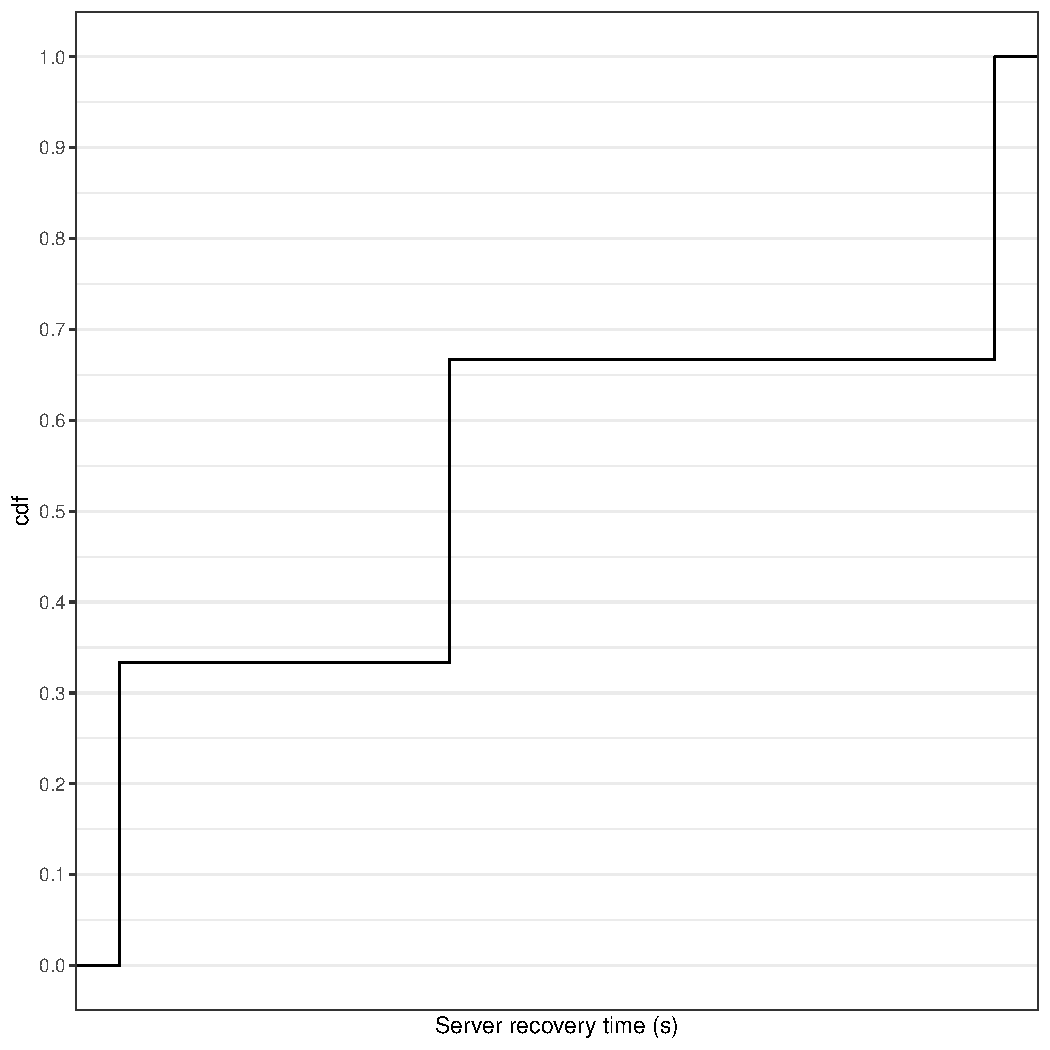
\includegraphics[keepaspectratio,width=\columnwidth]{server-recovery}
    \caption{Comparison of CDFs for server discovery between FlyWeb-based and Zeroties-based versions of Successorships.}
    \label{fig:eval:server-recovery}
\end{figure}

\section{Limitations and Future Work}
\label{sec:limitations_and_future_work}


\section{Related Work}
\label{sec:related_work}

\textbf{Zeroconf.}
Several researchers have investigated Zeroconf~\cite{Gunes2002, Bohnenkamp2003, Jara:2012:IPv6DNS-SD}.
For instance, \cite{hong2007accelerating} discusses that Zeroconf service discovery may cause overhead to the network while discovering new services.
Thus, they propose an algorithm to accelerate service discovery based on network topology changes.
Since a server failure would imply a change in the network topology, i.e. the server node being removed from the topology, 
client nodes in our implementation could use their approach to accelerate service discovery. 
Nonetheless, their implementation uses Linux Wireless extensions, which may not be accessible within a browser.
Thus, we used the FlyWeb service discovery implementation.

In~\cite{stolikj2016context}, Stolikj et al. argue that the number of published services in a network may also slow down service discovery.
As a solution, they propose a context-based approach, where queries specify which services they are interested in.
This approach is highly suitable for our work and we could use it to filter \APIshort services.
However, their approach changes service discovery queries and we question whether this could be easily integrated with existing devices.


\textbf{Local Networking APIs.}
Published in 2008, Universal Plug and Play (UPnP) is another widely-deployed set of networking protocols that facilitate discovery and interaction between devices on the same network, with minimal configuration.
Since it leverages common protocols (HTTP/XML/SOAP on UDP/IP) and is agnostic to the link medium, it is truly cross-platform, extending not only to phones and laptops but also to printers, WiFi routers, and audio-visual equipment, to name a few examples.
UPnP has been characterized as consisting of protocols that are more specific to particular classes of devices and applications; this is in contradistinction to Zeroconf, which aims to provide a device-agnostic foundation on which any device class or application-level protocol can build.~\footnote{\url{http://www.zeroconf.org/zeroconfandupnp.html}}

More recently in 2017, as part of its \textit{Nearby} project, \textit{Google} released its \textit{Connections} API, which enables Android devices in close proximity to one another to communicate in a peer-to-peer fashion.~\footnote{\url{https://developers.google.com/nearby/connections/overview}, accessed 2017-12-11}
This is done over a seamless mix of Bluetooth and WiFi hotspots.
Unfortunately, Google has only made this API available on the Android platform; we seek a solution that is truly cross-platform.

\textbf{In-browser web servers.}
An early example of fully in-browser web server technology was \textit{Opera Unite} (2009)\footnote{\url{http://help.opera.com/Windows/12.10/en/unite.html, accessed 2017-12-11}}.
This extension to the Opera browser enabled users to serve general-purpose Web applications directly from their browsers. 
Communication between clients and servers in this way could either be via Opera Unite's proxy servers, which also offered a name registering and directory service, or direct peer-to-peer, the latter requiring more advanced technical configuration.
Importantly, Opera Unite applications were constrained to be written as Opera ``Widgets''\footnote{An Opera Widget is an application that runs on Opera's now-deprecated Widget Engine, which allows such apps to be run independently of the browser.}.
Though the service was popular with a sizeable subset of Opera users, especially for purposes such as file sharing and media streaming, Opera eventually retired Unite in 2012 to consolidate the multiple extension frameworks offered in its browser.\footnote{http://www.instantfundas.com/2012/04/opera-to-discontinue-unite-widgets-and.html}

% TODO (PTC): Possibly add some notes on Web Server Chrome, and PeerServer.

\section{Conclusion}
\label{sec:conclusion}


\bibliographystyle{abbrv}
\bibliography{flyweb_paper}

\end{document}

